\section{Abstract}

\begin{singlespace}
Cranberries (\textit{Vaccinium macrocarpon}) are a high-value specialty crop, with the United States producing nearly 97\% of the global supply and Wisconsin contributing over 60\% of the domestic harvest \cite{usda-nass_cranberries_2024}. Monitoring cranberry growth and yield is particularly challenging because of the crop’s unique cultivation in sandy, low-lying marshes, the low stature of cranberry vines, and the small size of blossoms and fruit. Current monitoring approaches rely heavily on manual data collection or aerial imagery, which can be labor-intensive, inconsistent, or resolution-limited. This study presents the design and testing of a low-cost, ground-based robotic imaging platform tailored for cranberry research and smaller producers. The rover was designed to navigate sandy soils and narrow aisles in genetic phenotyping cranberry beds, collecting high-resolution RGB imagery of blossoms and fruit while minimizing disturbance to the crop. Field testing demonstrated the system’s robustness under variable conditions, capturing imagery suitable for bloom density assessment, yield estimation, and future machine learning applications. By offering an open-source, low-maintenance design that integrates autonomous navigation and precision imaging, this platform has the potential to expand access to advanced monitoring tools, reduce labor costs, and support data-driven management decisions in cranberry production.
\end{singlespace}

\newpage

\section{Introduction}

The integration of robotic imaging technology into agriculture is transforming how crops are monitored and managed by providing precise, real-time data on plant health, growth stages, and yield estimation \cite{cinat_comparison_2019}. Ground-based robotic rovers equipped with RGB, multispectral, and hyperspectral cameras can collect high-resolution imagery under consistent conditions, overcoming many of the altitude and lighting limitations of aerial platforms \cite{wendel_self-supervised_2016}. When combined with computer vision and machine learning algorithms, these systems have shown promise for detecting plant stress \cite{abebe_image-based_2023}, quantifying flowering, and improving yield predictions with greater accuracy than traditional sampling methods.

While these advances are well documented in crops such as tomatoes \cite{seo_development_2021}, lettuce \cite{hu_lettucetrack_2022}, and peppers \cite{lehnert_autonomous_2017}, specialty crops like cranberries present unique challenges. Cranberries are grown in sandy, acidic marshes across northern U.S. states, with Wisconsin and Massachusetts accounting for the majority of production \cite{usda-nass_cranberries_2024}. Unlike orchard or row crops, cranberries form low, vine-like mats with blossoms and fruit borne close to the ground \cite{sandler_cranberry_2008}. Monitoring bloom density and berry set is labor-intensive and prone to sampling error, yet these factors directly influence pollination success and yield. Furthermore, cranberry production faces persistent threats from fungal fruit rot complexes and insect pests, where timely detection and intervention are critical \cite{oudemans_cranberry_1998}.

Despite advances in robotics for other crops, cranberry monitoring remains reliant on on manual field scouting or aerial imagery, both of which present limitations. Manual scouting is time-consuming and constrained in spatial coverage, while aerial imagery often lacks the resolution necessary to detect individual cranberry flowers or small fruits. These unique agronomic and environmental conditions create an opportunity for lightweight, ground-based robotic rovers that can provide consistent, high-resolution data without damaging the crop.

This study presents the development and field validation of a purpose-built robotic rover designed to meet these challenges. The platform integrates high-resolution imaging, autonomous navigation, and robust frame design into a compact system optimized for cranberry marsh conditions. By addressing the barriers of cost, usability, and crop-specific constraints, the system aims to expand access to precision agriculture technologies for small and mid-sized cranberry producers, enabling more efficient bloom monitoring, improved yield estimation, and enhanced long-term crop management.


\section{Design}

The UGV was designed to traverse the grid system of test plots using the separation aisles between plots in order to minimize disturbance to the plants. Navigating the marsh proved to be a challenging task while providing a stable imaging platform. Any unnecessary disturbance needed to be avoided as it would potentially affect flower pollination. To improve overall mobility, a wheeled skid-steering type rover was chosen. This choice allowed the use of large diameter wheels necessary to navigate the sandy soil type while still allowing the rover to perform pivot-style turns at the end of each grid column.

\subsection{Frame}
The rover was modeled in Creo Parametric \cite{ptc_creo_2023} with multiple revisions considered. To allow for easier modification, the frame was designed with primarily bolted connections. This allows for modification of dimensions as well as changing out entire sections of the robot. An isometric view of the model can be seen in Figure~\ref{fig:Initial CAD Model}. Steel was chosen for the primary frame material due to its low relative cost and ease of manufacture. Aluminum was used for auxiliary brackets and supports including the camera mount. Although the steel structure resulted in an increased weight compared to an aluminum frame, the total weight of the frame excluding wheels and electronics was relatively low at 72 lbs. Considering the entire weight of the robot of 138 lbs, the frame only accounts for less than 60\% of the total weight.


\begin{figure}[!ht]
    \centering
    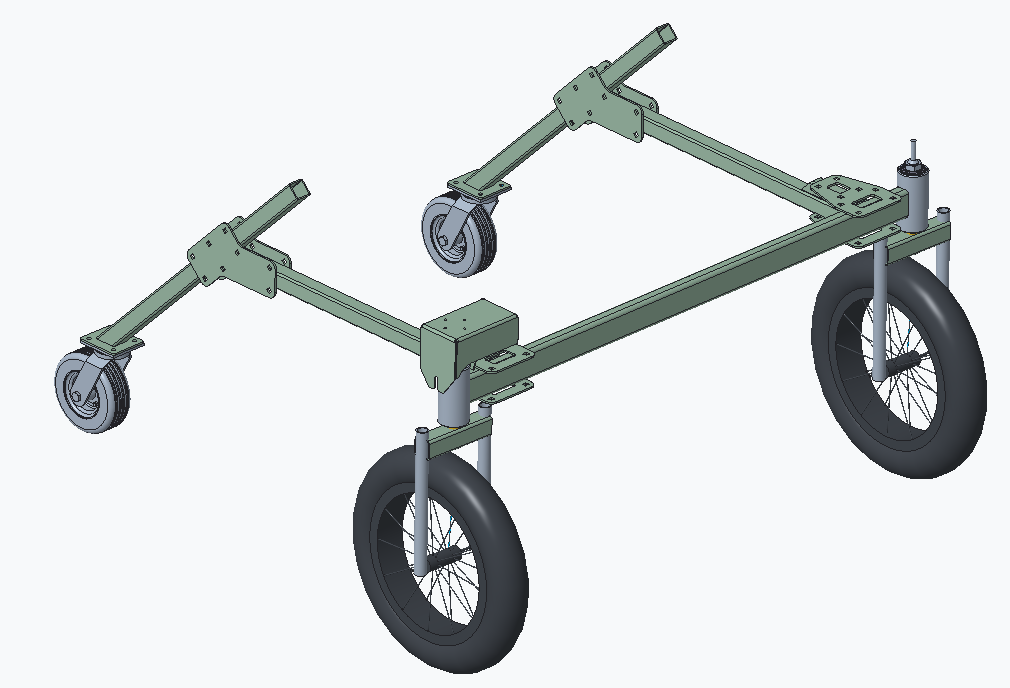
\includegraphics[width=0.75\linewidth]{images/CAD.png}
    \caption{Autonomous rover—3D CAD overview. The isometric view shows the two-wheel differential-drive layout with steerable front wheels. Note all joints between the front drive wheels and rear caster wheels are accomplished with bolted plates}

    \label{fig:Initial CAD Model}
\end{figure}

Control and steering were considered as likely systems to need to be tested and modified, so two systems were implemented in the initial design. The primary system was a differential steering system; this style  was chosen as it would provide simple control as well as good maneuverability. The secondary system was a pivoting wheel system where the main drive wheel could be rotated relative to the vehicle frame as seen in Figure~\ref{fig:steer}. This system would allow the main wheels to be pivoted around their vertical axis independently, controlled by a stepper motor (23HS22-5004D-E1000, STEPPERONLINE, China) attached to a NEMA 23 10:1 worm drive gearbox (Generic, China). A stepper motor was chosen for its low power consumption, and when coupled with a worm drive gearbox, this would allow the robot to maintain the steering position with no additional power due to the worm drive gearbox's self-locking characteristics.

\begin{figure}
    \centering
    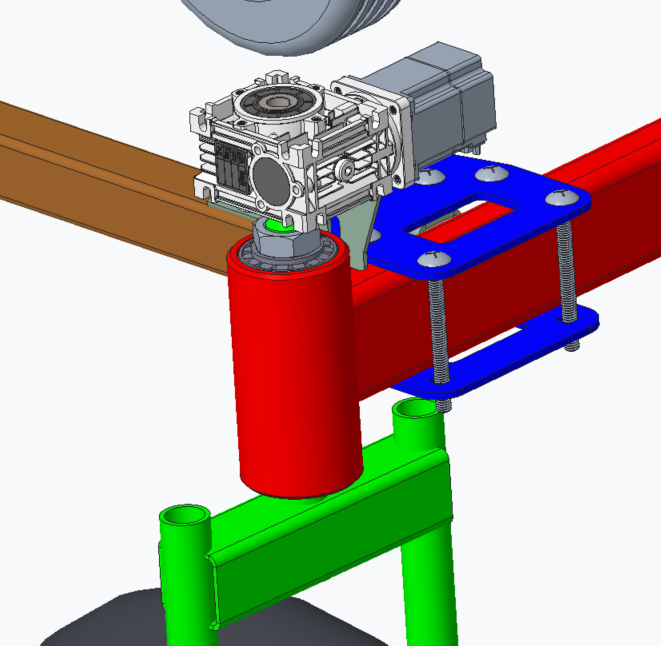
\includegraphics[width=0.75\linewidth]{images/secondary steering.png}
    \caption{Steering motor and gearbox assembly. A NEMA-23 stepper coupled to a 10:1 worm gearbox provides self-locking hold torque, allowing precise steering without continuous power draw. The assembly mounts above the drive axis for easy servicing and keeps moving parts clear of vegetation.}

    \label{fig:steer}
\end{figure}

\subsection{Sensing platform}

Two imaging systems were investigated, the first being a RealSense D435i (Intel, USA) and the second being a Canon PowerShot A810a (Canon U.S.A, USA). The Canon digital camera was selected due to better performance in most lighting conditions as well as a significantly higher image resolution. The camera was able to be interfaced with the UGV controller. The Canon captured a 16MP RGB image of size 4608 px $\times$ 3456 px and a maximum field of view of 65 degrees.  Images were captured at a height of 1500 mm and with the field of view controlled such that an area approximately 1200 mm $\times$ 1700 mm was captured. This FOV and image resolution gave a ground sampling distance (GSD) of approximately 0.37 mm/px. This resolution was chosen as a typical blossom was found to be approximately 6.3 mm to 9.5 mm \cite{diaz-garcia_image-based_2018}, with some features such as individual petals being smaller. The combination of flower size and GSD ensured approximately 15-20 pixels per flower. Images were captured using natural lighting in early afternoon to provide minimal self-shadowing and to avoid shadowing from the image collection platform.


The consideration of image lighting was a major concern to ensure that the images were as uniform as possible before any analysis was performed. The images were collected in full and partial sun as well as under a canopy that blocked all direct and ambient sunlight and used controlled artificial lighting. The best results were found using natural lighting with a solar elevation angle roughly equal to the field of view of the camera system.
    
\begin{figure}[!ht]
  \begin{subfigure}{0.3\textwidth}
    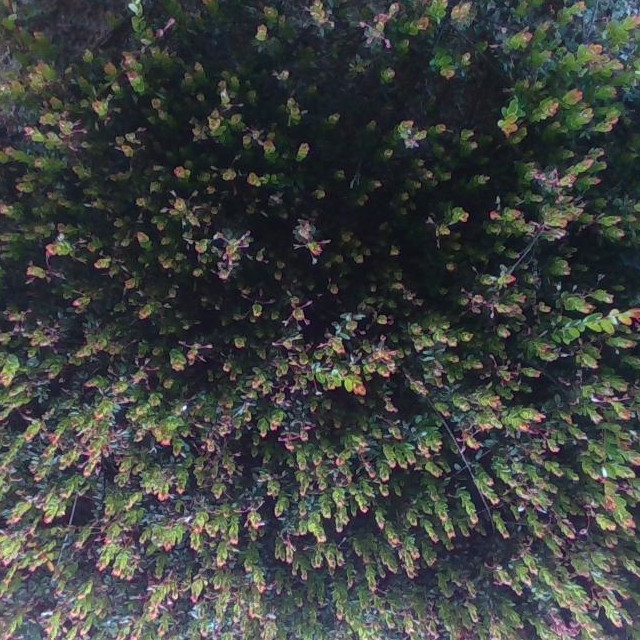
\includegraphics[width=\textwidth]{images/No-Light_7-119.JPG}
   \caption{Shaded Image}
    \label{fig:NoLight}
  \end{subfigure}
  \hfill
  \begin{subfigure}{0.3\textwidth}
    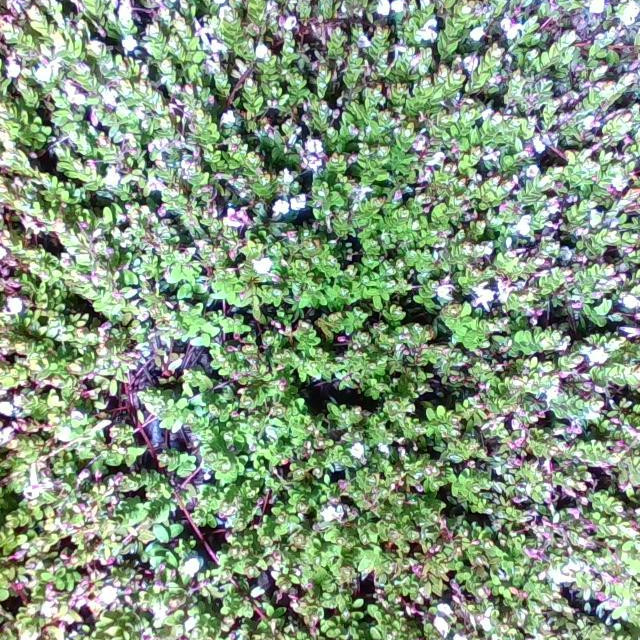
\includegraphics[width=\textwidth]{images/Artficial-Light_7-119.JPG}
   \caption{Artificial Lighting}
    \label{fig:ArtficialLight}
  \end{subfigure}
  \hfill
  \begin{subfigure}[b]{0.3\textwidth}
    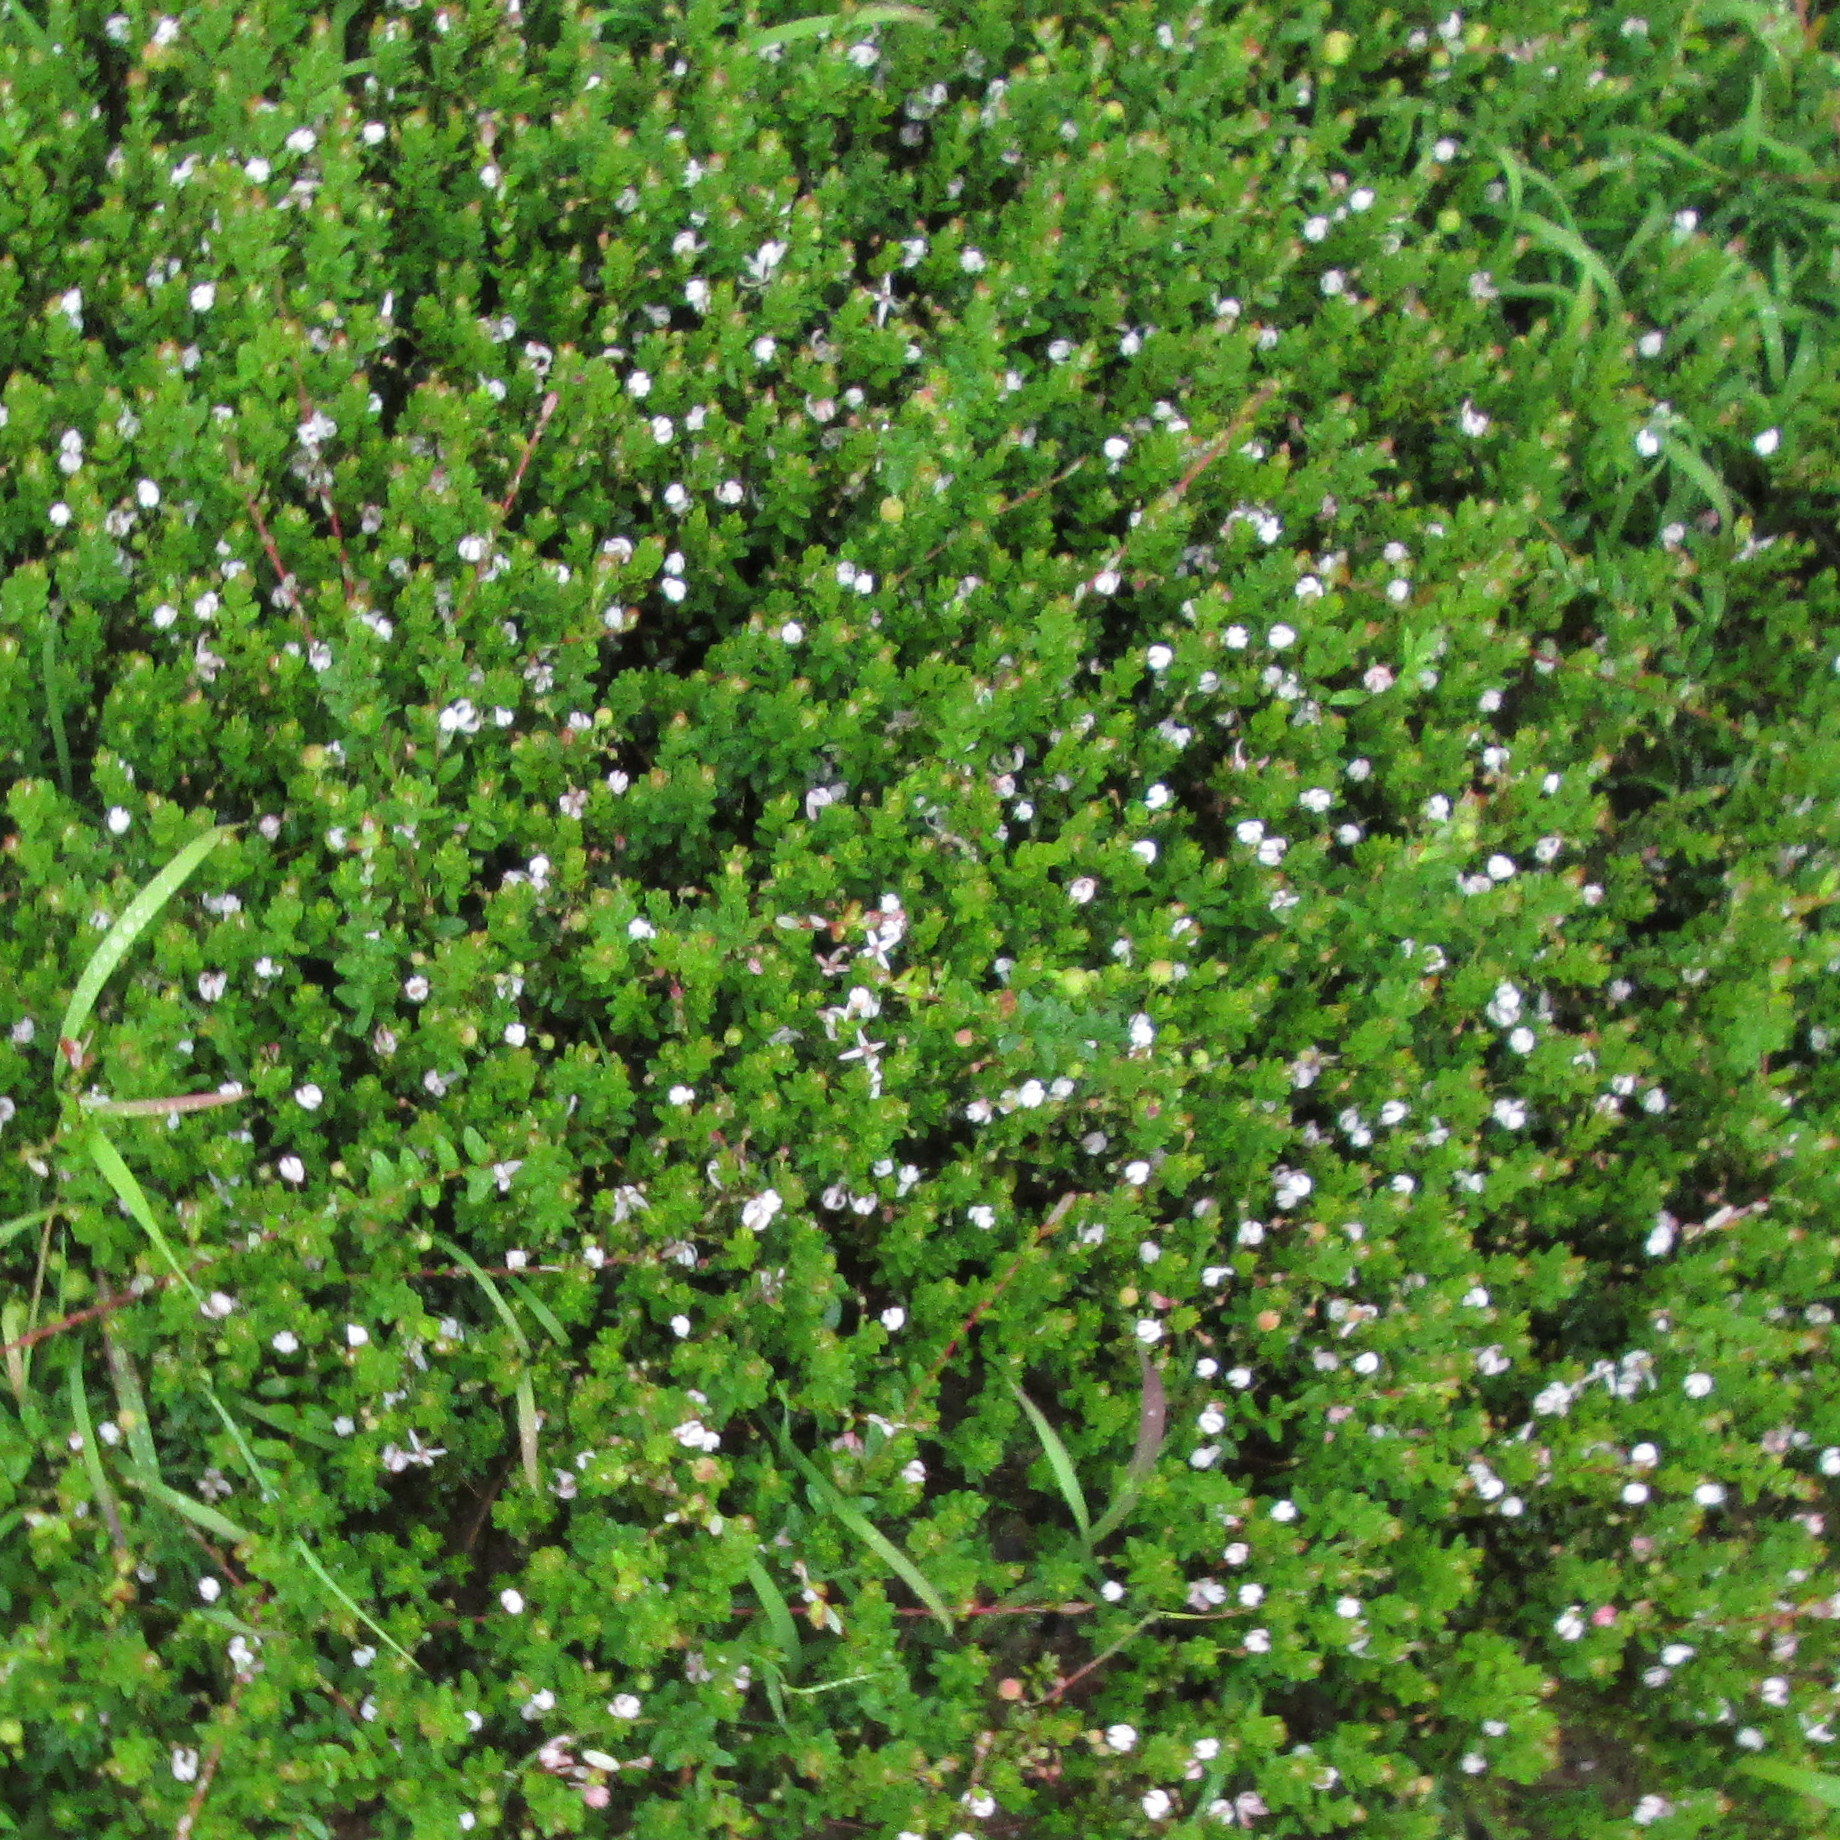
\includegraphics[width=\textwidth]{images/Nat_light_7-119.JPG}
    \caption{Natural Lighting}
    \label{fig:NaturalLight}
  \end{subfigure}
  \caption{Lighting conditions evaluated for image collection. (a) Shaded imaging reduces highlights but lowers contrast on floral structures. (b) Artificial lighting under a canopy yields stable exposure but introduces color cast and specular artifacts on glossy leaves. (c) Natural sunlight with mid-day solar elevation gave the most consistent separation of petals and foliage at our working height, so it was adopted for the main survey.}

  \label{fig:LightComp}
\end{figure}
    
In an effort to further minimize shadowing, the camera was mounted remotely to the A-UGV on an elevated arm in front of the primary structure, as shown in Figure~\ref{fig:CamMount}. The path of the A-UGV could also be optimized to avoid producing interfering shadows; typically, this was realized by traveling in a North-South direction, thus shadows produced were to the left or right of the plot being imaged.

\begin{figure}[!ht]
  \begin{subfigure}{0.4\textwidth}
    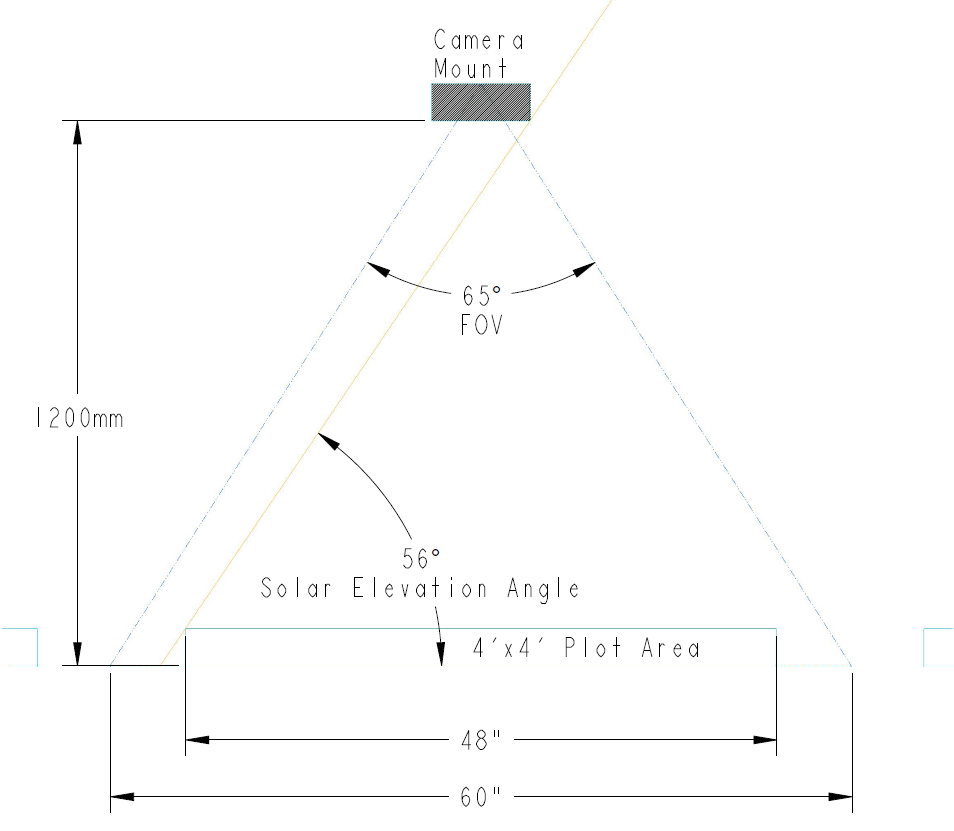
\includegraphics[width=\textwidth]{images/Sun Angle.png}
   \caption{Solar elevation relative to camera}
    \label{fig:SolAng}
  \end{subfigure}
  \hfill
  \begin{subfigure}[b]{0.4\textwidth}
    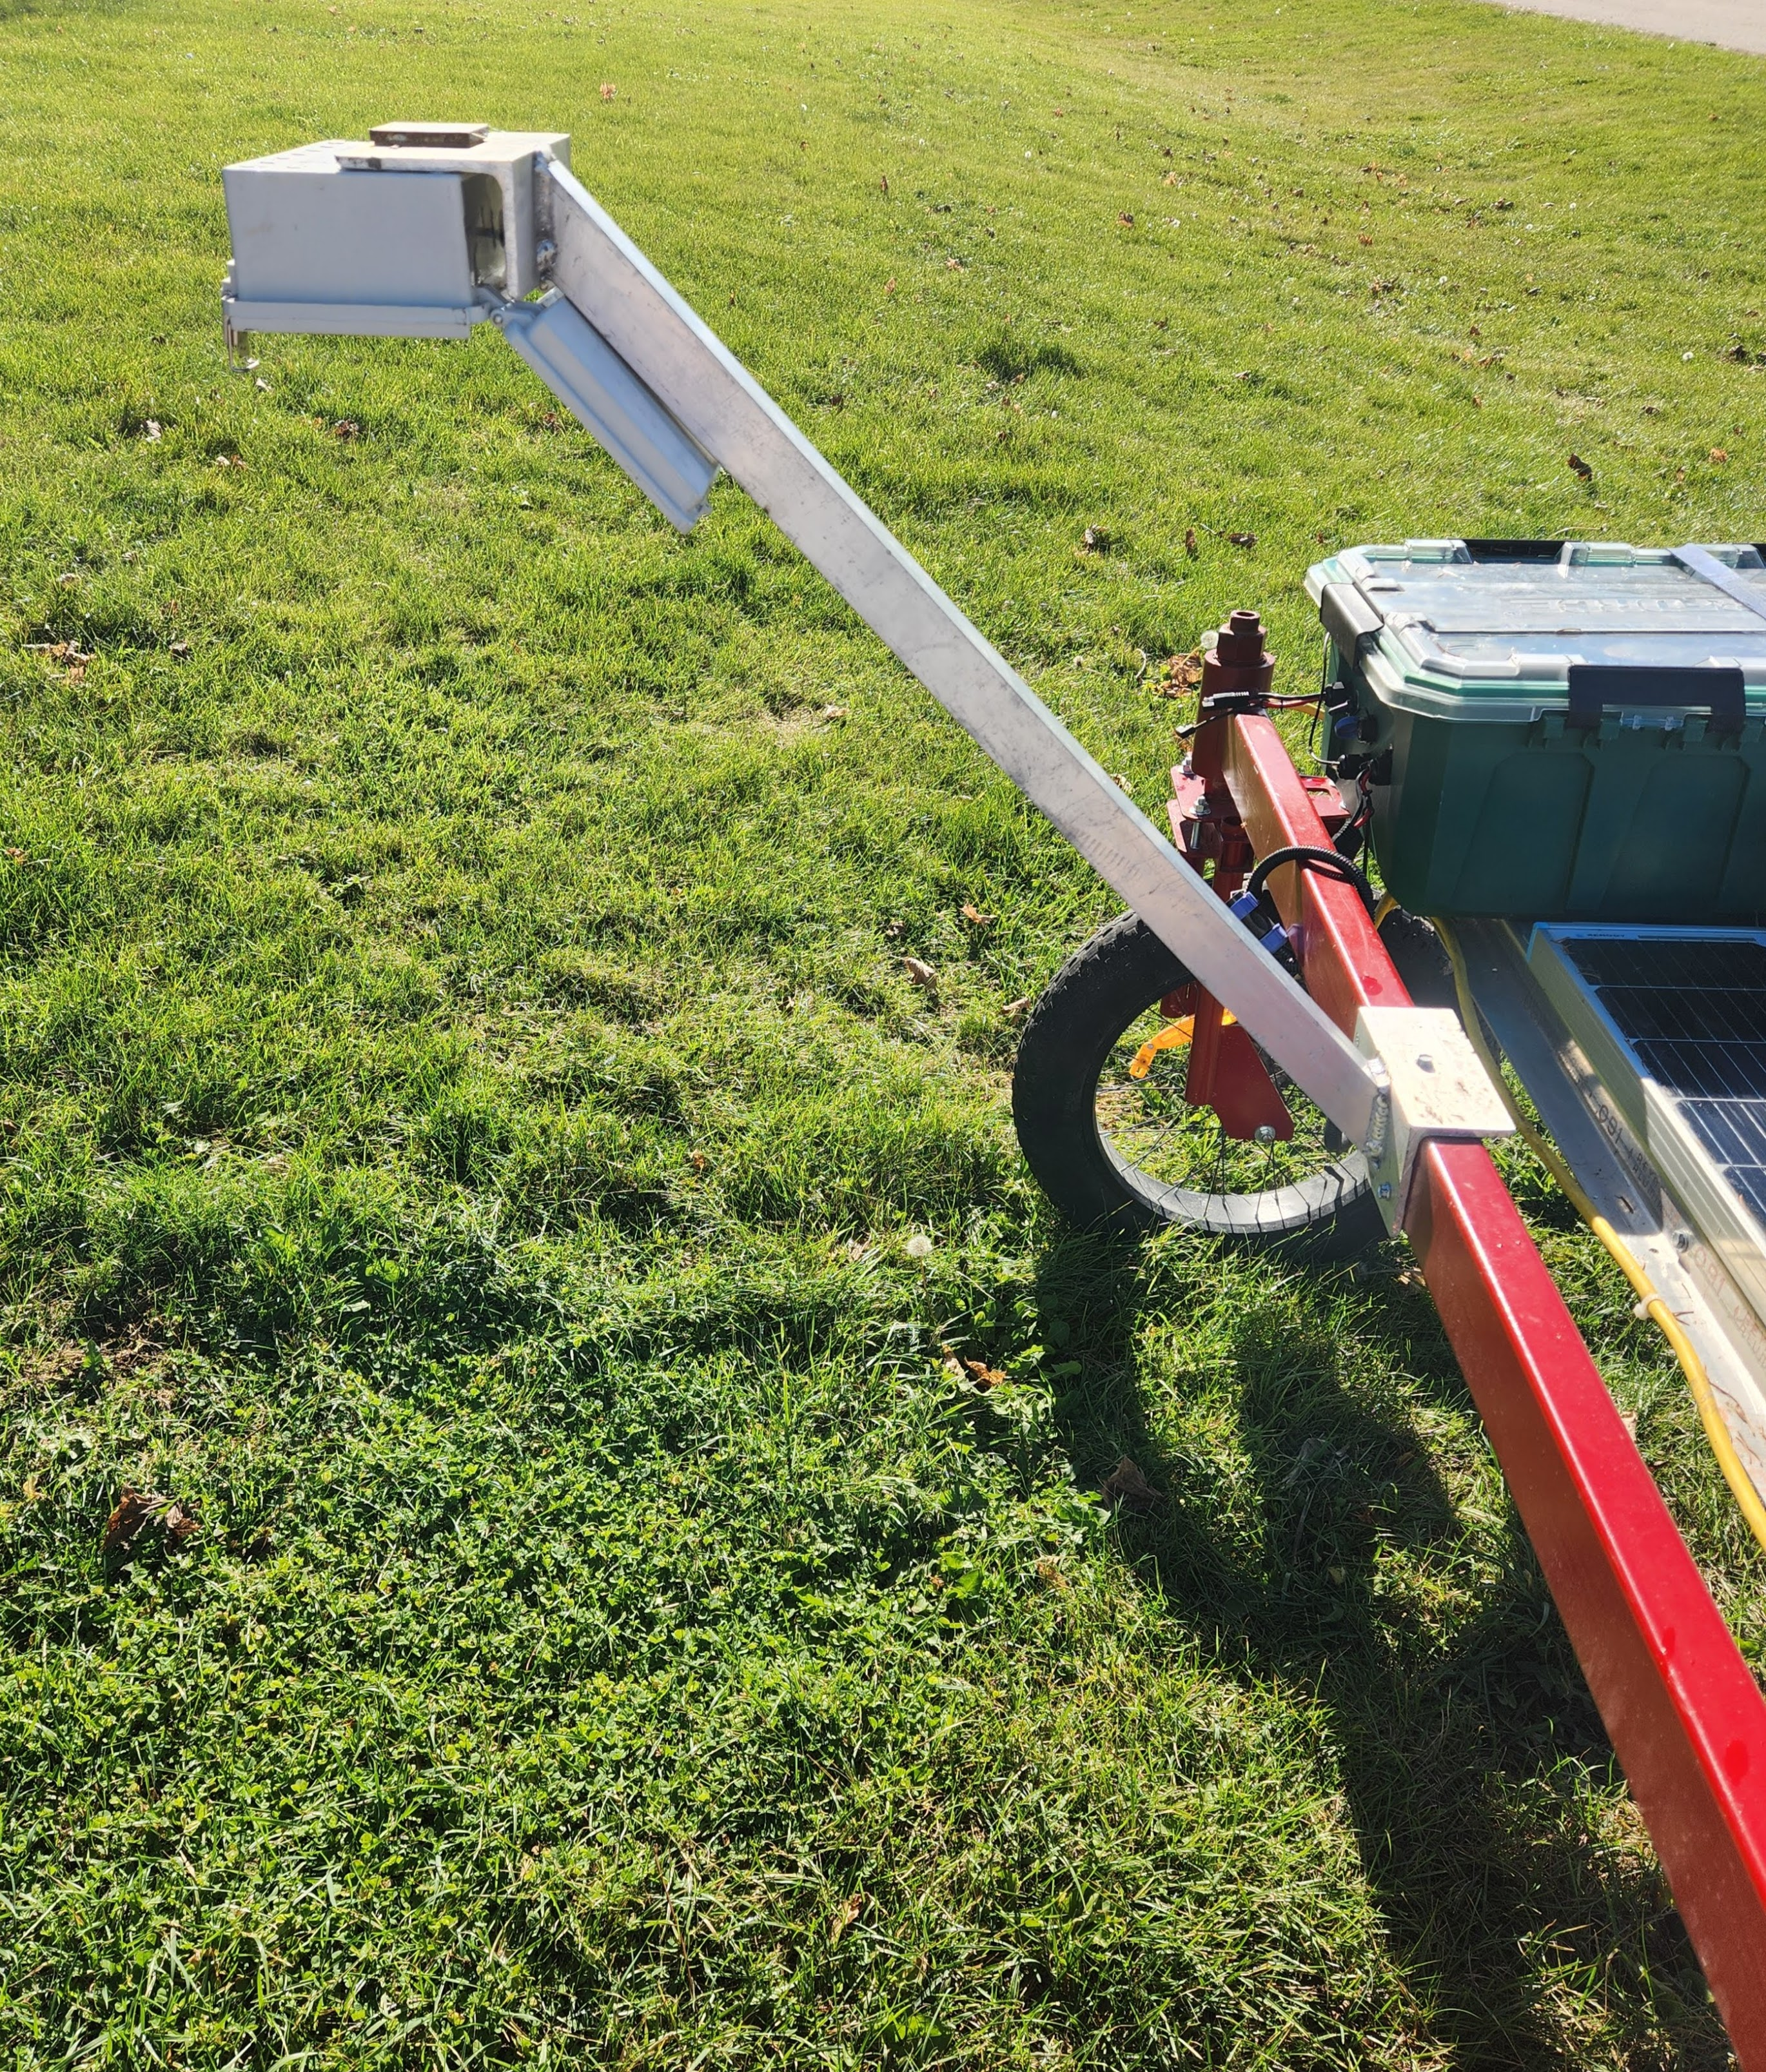
\includegraphics[width=\textwidth]{images/Camera Mounting.jpg}
    \caption{Remote Camera Mount}
    \label{fig:CamMount}
  \end{subfigure}
  \caption{Shadow mitigation strategy. (a) Operating when the solar elevation roughly matches the camera field of view minimizes casting of shadows into the plot. (b) A forward, elevated camera mount places optics ahead of the chassis so any residual shadows fall outside the FOV area. Together these choices improved mask quality and reduced false detections.}

  \label{fig:ShadowMit}
\end{figure}


\subsection{Electronics and Control}

After the completion of the hardware to be used on the sensing platform, the electronics and power system were next selected and implemented.

Current agricultural robotics commonly rely on either electrical or hydraulic power depending on the tasks performed. Hydraulic systems are typically of higher power output and often coupled to internal combustion engines as primary movers. This increased power makes them well suited for and used in seeding and weeding or tilling operations \cite{vahdanjoo_operational_2023}. Lower power systems that typically see use in imaging or crop sensing are often powered by electrical systems as this simplifies maintenance and increases field endurance as they can often be supplemented with recharging areas or solar power \cite{quaglia_design_2020}

For our design, a robust and efficient system is required due to the challenging conditions seen in the cranberry bog the robot would be operating. A particular focus was put onto both heat and water resistance due to the season of sampling, mid to late summer, as well as the use of irrigation in the field. For reasons discussed above, an electrical power system was selected. Thanks to recent advancements, the availability of lithium-ion batteries has greatly improved and is commonly used on other agricultural robotic platforms. \cite{ghobadpour_off-road_2022} A self-contained system that integrates both the lithium cells as well as a battery management system (BMS) was selected; this allowed easier service and replacement if needed. The batteries selected were a Timeusb 12V 50Ah, and (2) battery banks rated at 12 volts nominally were run in series to provide 24 volts to the system as shown in figure~\ref{fig:Battery System}. 

\begin{figure}[!ht]
    \centering
    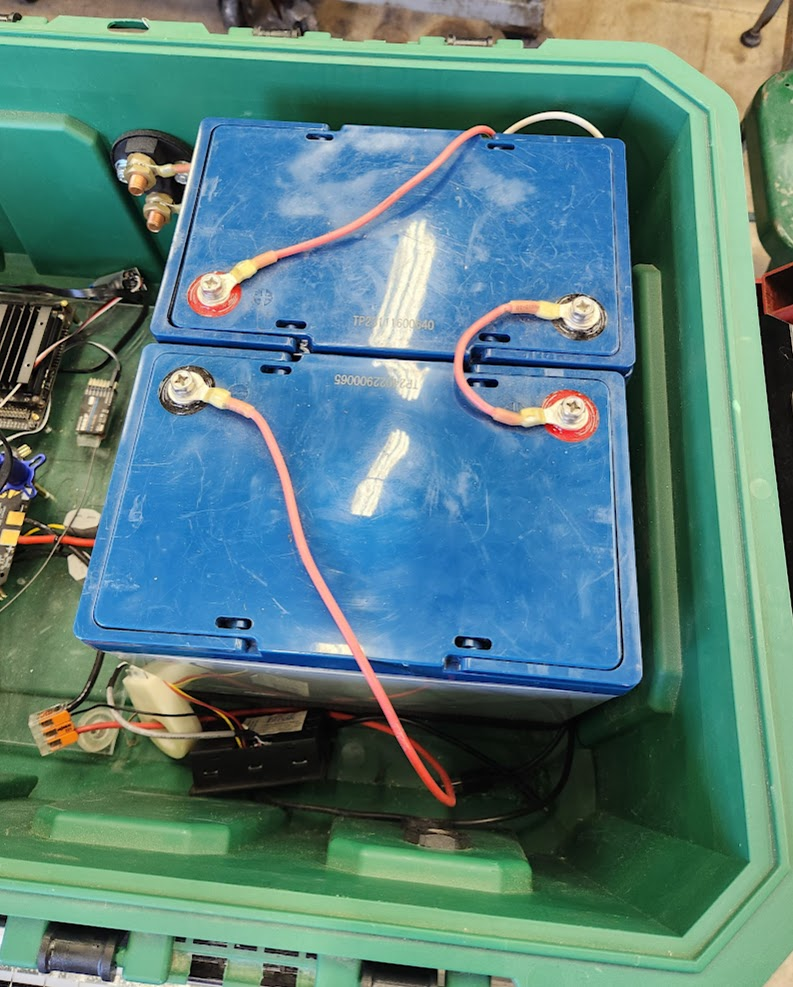
\includegraphics[width=0.5\linewidth]{images/Batteries.jpg}
    \caption{Onboard power system. A LiFePO\textsubscript{4} battery pack in a weather-sealed case supplies power for the controller, compute module, and sensors. The battery pack selected is fully self contained including a internal BMS.}
    \label{fig:Battery System}
\end{figure}

A capacity of 50 amp-hours was selected based on initial calculations using a conservative estimated load of 250 Watts, consumed primarily by the drive motors, at a voltage of 24 volts; nominally, this correlated to a current load of approximately 20.8A.

\begin{equation}
    \frac{250 \, \text{W}}{24 \, \text{V}} = 10.4 \, \text{A}
    \label{eq:power_equation}
\end{equation}

Using this amp loading and an estimated sampling time of 1.5 hours for 360 plots with a sample interval of 15 seconds per plot gave a total energy usage of 15.6 amp-hours, at a nominal voltage of 24 volts this equates to approximately 375 W-hours. The total energy stored by the battery system is approximately 1200 W-Hours. This additional capacity also allows for future expansion and inclusion of additional sensors that may require additional power during operation. In addition to the power storage of the batteries, a solar panel was fitted that provided a maximum of 100 watts to the system. Based on an estimated global horizontal irradiance of 6.1 kWh/m2/day\cite{nrel_pvwatts_2024} and a panel output of 100 Watts the power produced will be approximately 500 W-Hr daily providing the rover with enough energy to fully recharge the energy lost during sampling.

\begin{figure}[!ht]
    \centering
    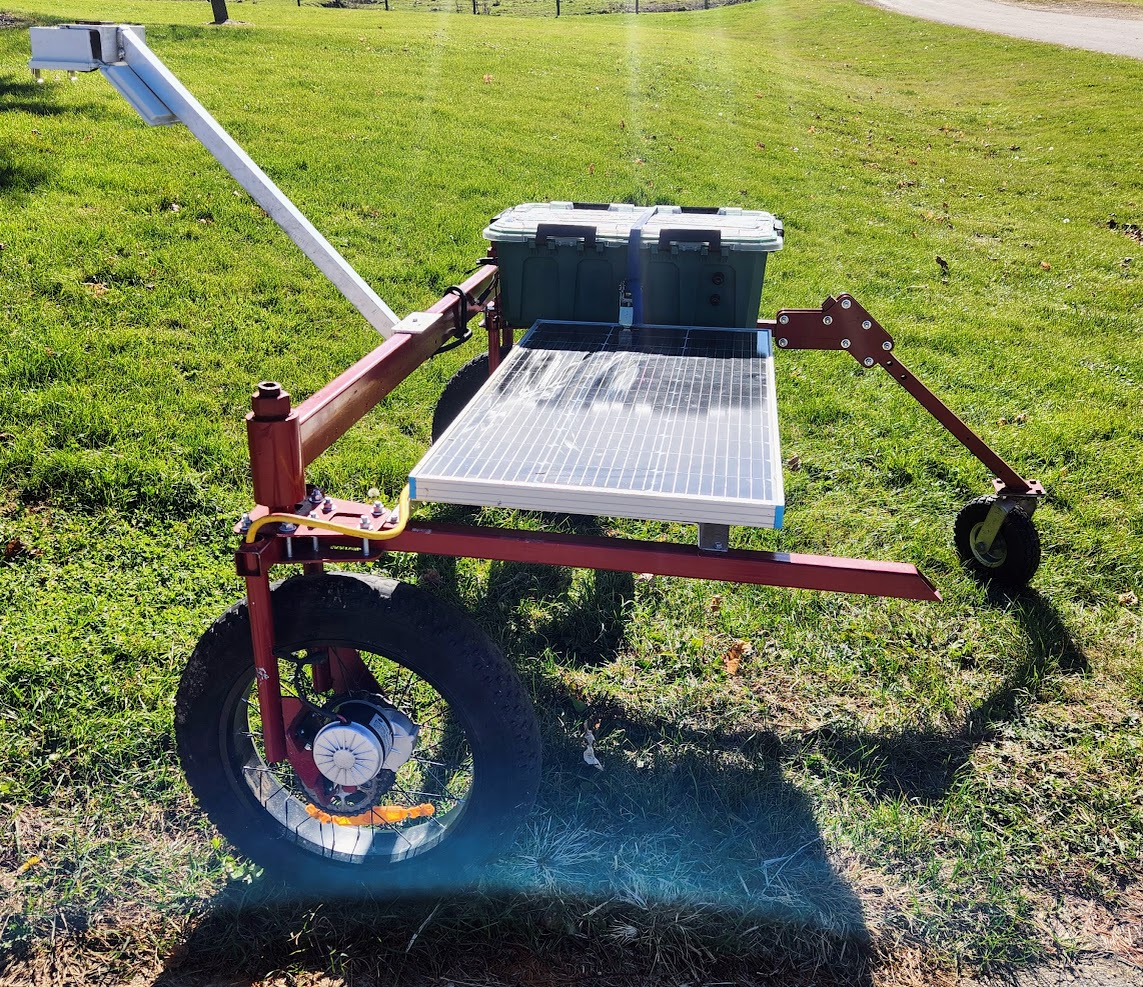
\includegraphics[width=0.5\linewidth]{images/Solar Panel.jpg}
    \caption{100\,W solar replenishment on rover. A panel mounted above the chassis slowly charges the main pack during idle and low-load transits, extending run time across multi-hour sampling sessions.}
    \label{solar-panel}
\end{figure}

The next component selected was the physical ground drive system. Again, multiple options were evaluated before selection. For the ground engaging components, the systems considered were a continuous rubber track or a wheeled drive. While tracks provided decreased ground pressure and improved tractive force, there was concern that turning may disturb the trackways between plots, and it was determined to use 2 20" diameter 4" wide bicycle wheels as the primary ground engaging component. For propulsion, 2 brushed 250W motors, one on each wheel, were used and connected via a chain drive as shown in Figure~\ref{fig:Wheel and drive}. This drive system was simple and would still allow the gearing between the motor and the wheel to be adjusted.

\begin{figure}[!ht]
    \centering
    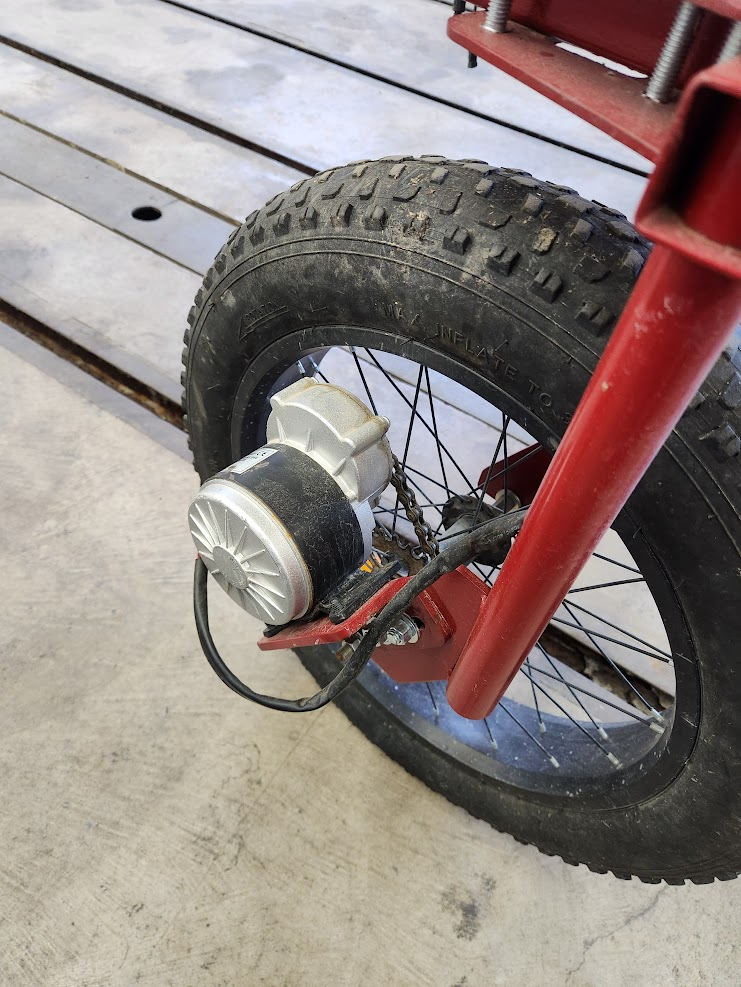
\includegraphics[width=0.5\linewidth]{images/Drive Wheel.jpg}
    \caption{Drive wheels and chain transmission. Two 20\,in pneumatic bicycle wheels driven by 250\,W brushed motors provide traction on soft sand and organic matter typical of cranberry beds. The simple chain reduction allows quick gearing changes to trade speed for torque as needed.}
    \label{fig:Wheel and drive}
\end{figure}

After specifying and assembling all the physical components, the electronic control system was required. Again, reviewing current offerings and maintaining a focus on using commercially available components led to the selection of a consumer-based flight control system. A CubePilot (CubePilot, Australia) flight controller (FC) was selected and mounted to a CubePilot Kore Carrier Board. This system was desirable due to its including many of the necessary auxiliary systems such as a breakout connector for sensors and general-purpose input/output (GPIO) headers.

\begin{figure}[!ht]
    \centering
    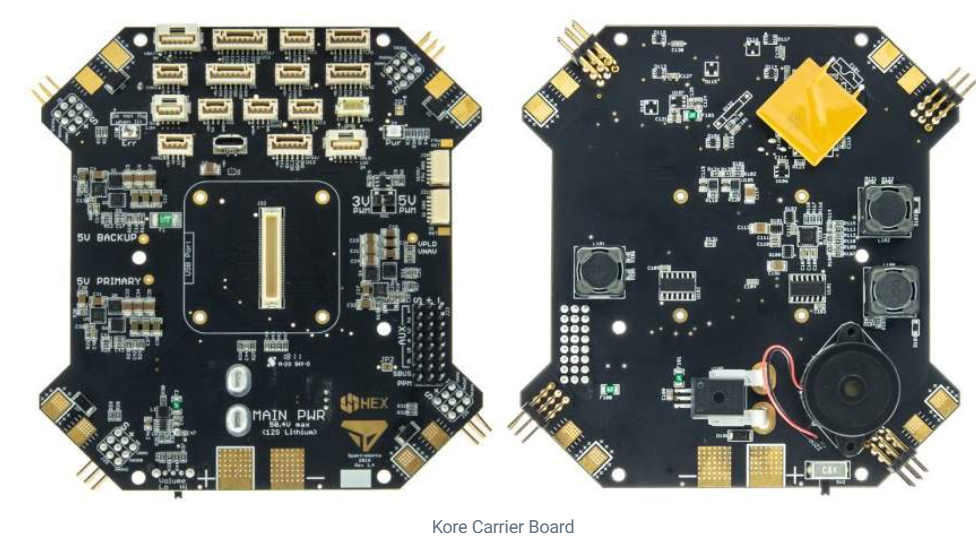
\includegraphics[width=0.5\linewidth]{images/Kore Carrier.png}
    \caption{CubePilot Kore carrier board. The board consolidates power management, sensor breakouts, and GPIO headers for the CubePilot flight controller used here as the rover’s navigation and I/O computer. This off-the-shelf stack reduced custom wiring and improved reliability.}
    \label{fig:Carrier board}
\end{figure}

Multiple solutions were considered for primary navigational data, including vision-based, laser-guided, and RTK GPS. After evaluation, RTK GPS was found to be the most suitable due heavily to its ease of implementation as well as accuracy to sub-inch levels. Two systems were used to increase redundancy. The primary system was a system produced by Emlid (Emlid, Hungary) Reach M2 UAV RTK Kit. This kit includes a base station that uses a Long Range (LoRa) radio unit to send correction data to the rover as shown in Figure~\ref{fig:Local Corection RTK}.

\begin{figure}[!ht]
    \centering
    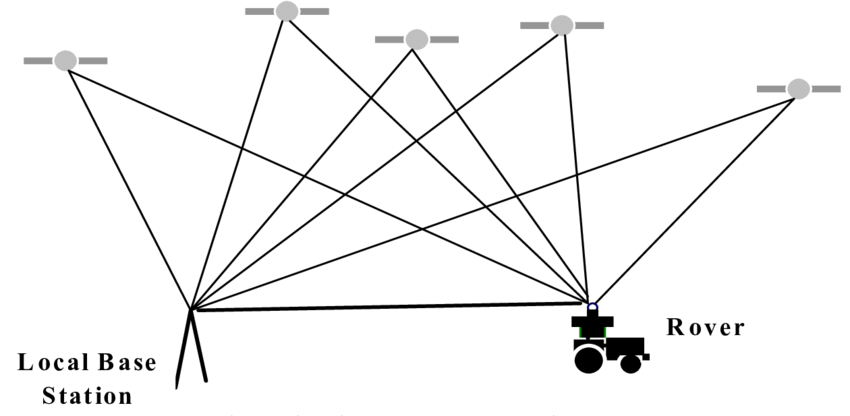
\includegraphics[width=0.5\linewidth]{images/RTK-GPS.png}
    \caption{RTK system with local base station. An Emlid Reach M2 base broadcasts RTCM corrections over LoRa to the rover receiver, enabling sub-inch positioning for plot alignment. This mode was used when on-site base setup was feasible and radio line-of-sight was reliable.}
    \label{fig:Local Corection RTK}
\end{figure}

The second system is a SparkFun GPS-RTK2 development board (SparkFun, USA) that uses a ZED-F9P module by UBlox (UBlox, Switzerland). This system uses a Networked Transport of RTCM via Internet Protocol (NTRIP) service for corrections provided by the Wisconsin Continuously Operating Reference Station (WISCORS) operated by the Wisconsin Department of Transportation. The WISCORS system works by collecting and combining atmospheric correction data from 115 stations throughout the state and providing correction data through a web application available to the public\cite{wisconsin_department_of_transportation_wiscors_nodate}. 

\begin{figure}[!ht]
    \centering
    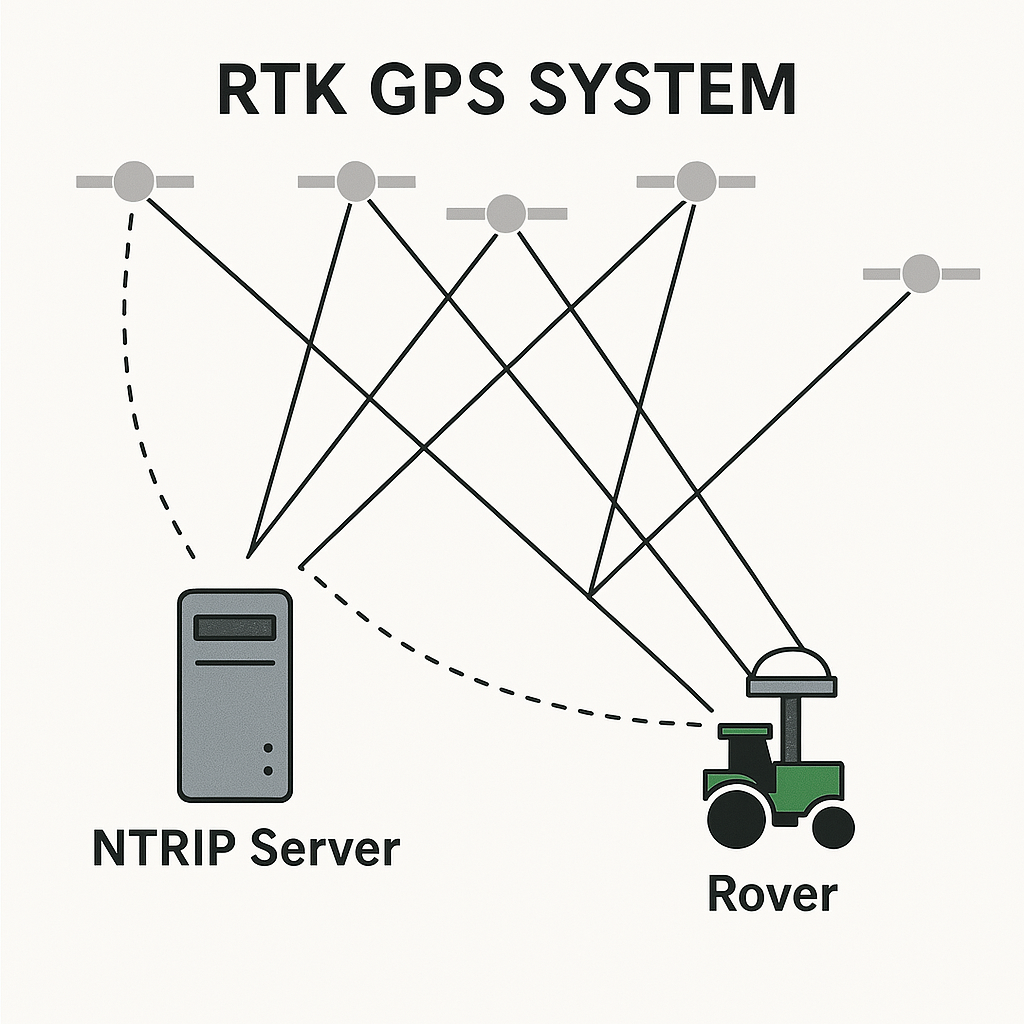
\includegraphics[width=0.5\linewidth]{images/Ntrip.png}
    \caption{RTK via NTRIP corrections. A ZED-F9P receiver on the rover obtains state-wide corrections from the WISCORS network over internet accessable data. This configuration provided a no-base alternative with comparable accuracy when infrastructure access was available.}
    \label{fig:NTRIP RTK}
\end{figure}

To control and program the physical rover unit, a ground station was used. We used the Open Source Software package Mission Planner ver 1.3.82, maintained by the ArduPilot team \cite{ardupilot_mission_nodate}. This allowed us to both program parameters into the rover used in navigation and control, as well as upload specific missions used for path planning and waypoint creation during the data collection.

\begin{figure}[!ht]
    \centering
    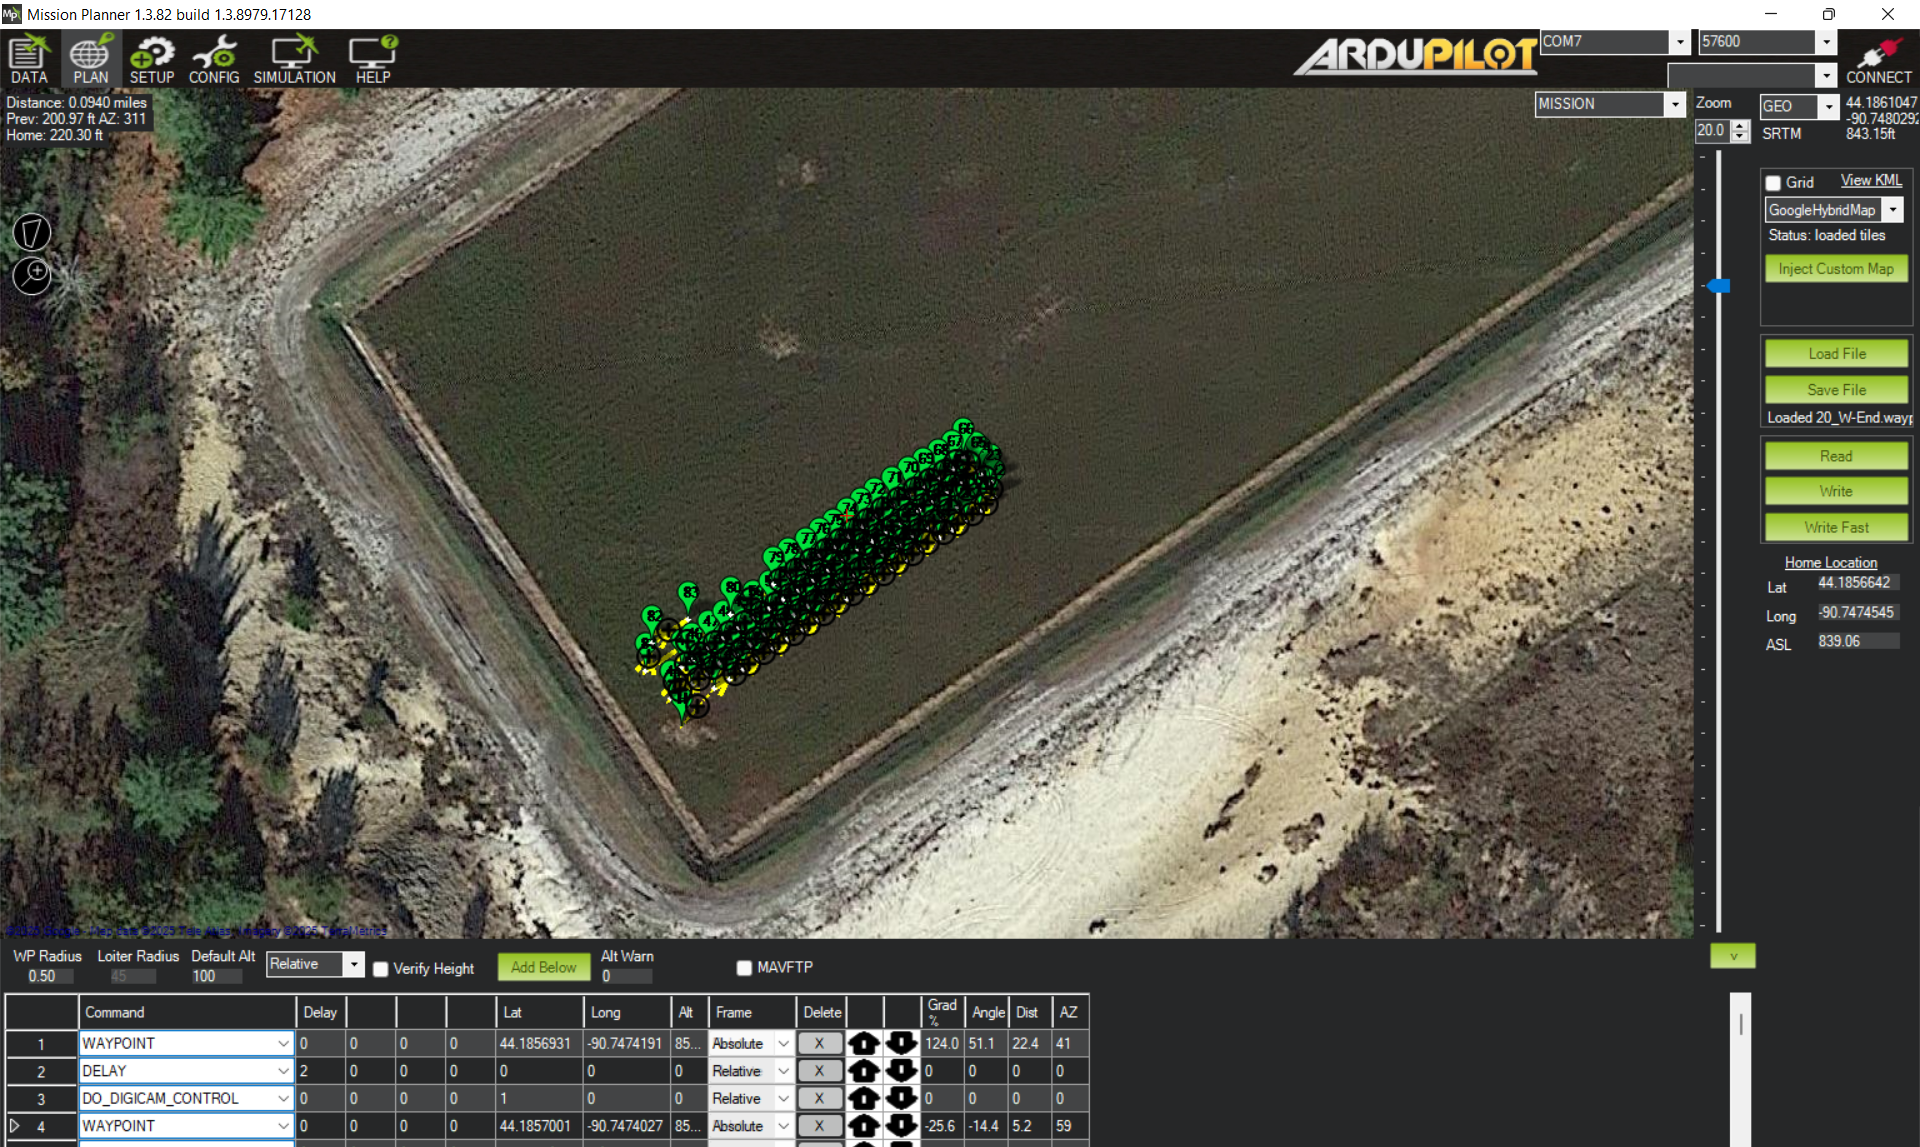
\includegraphics[width=0.5\linewidth]{images/Mission Planner.png}
    \caption{Mission Planner ground-station interface. The operator configured rover parameters, uploaded waypoint missions, and logged GNSS status through this interface. Using a repeatable mission file ensured consistent plot coverage across collection days.}
    \label{fig:Mission Planner}
\end{figure}

\section{Testing}

Plots were surveyed 2 times, once with a handheld RTK receiver placed at the center of each plot on the East End of the field and once using the rover. To use the rover for surveying, it was manually piloted to be centered over the plot and then triggered to record its position as a way-point in the mission planner software. This technique was able to produce a high-quality map of desired way-points without additional processing and removed potential errors during translation between hardware setups.

\begin{figure}[!ht]
    \centering
    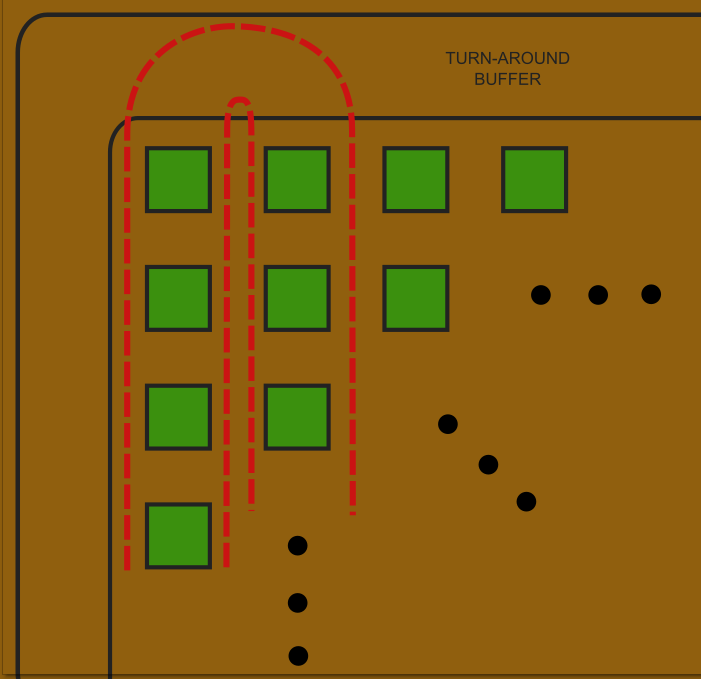
\includegraphics[width=0.5\linewidth]{images/TurnAround.png}
    \caption{Robot path navigation for plot coverage. Waypoints were centered over each plot; turns used buffer lanes to avoid driving through imaged plant canopies. The repeatable path minimized trampling, reduced navigation time, and kept imaging geometry consistent.}
    \label{fig:path}
\end{figure}

\begin{figure}[!ht]
    \centering
    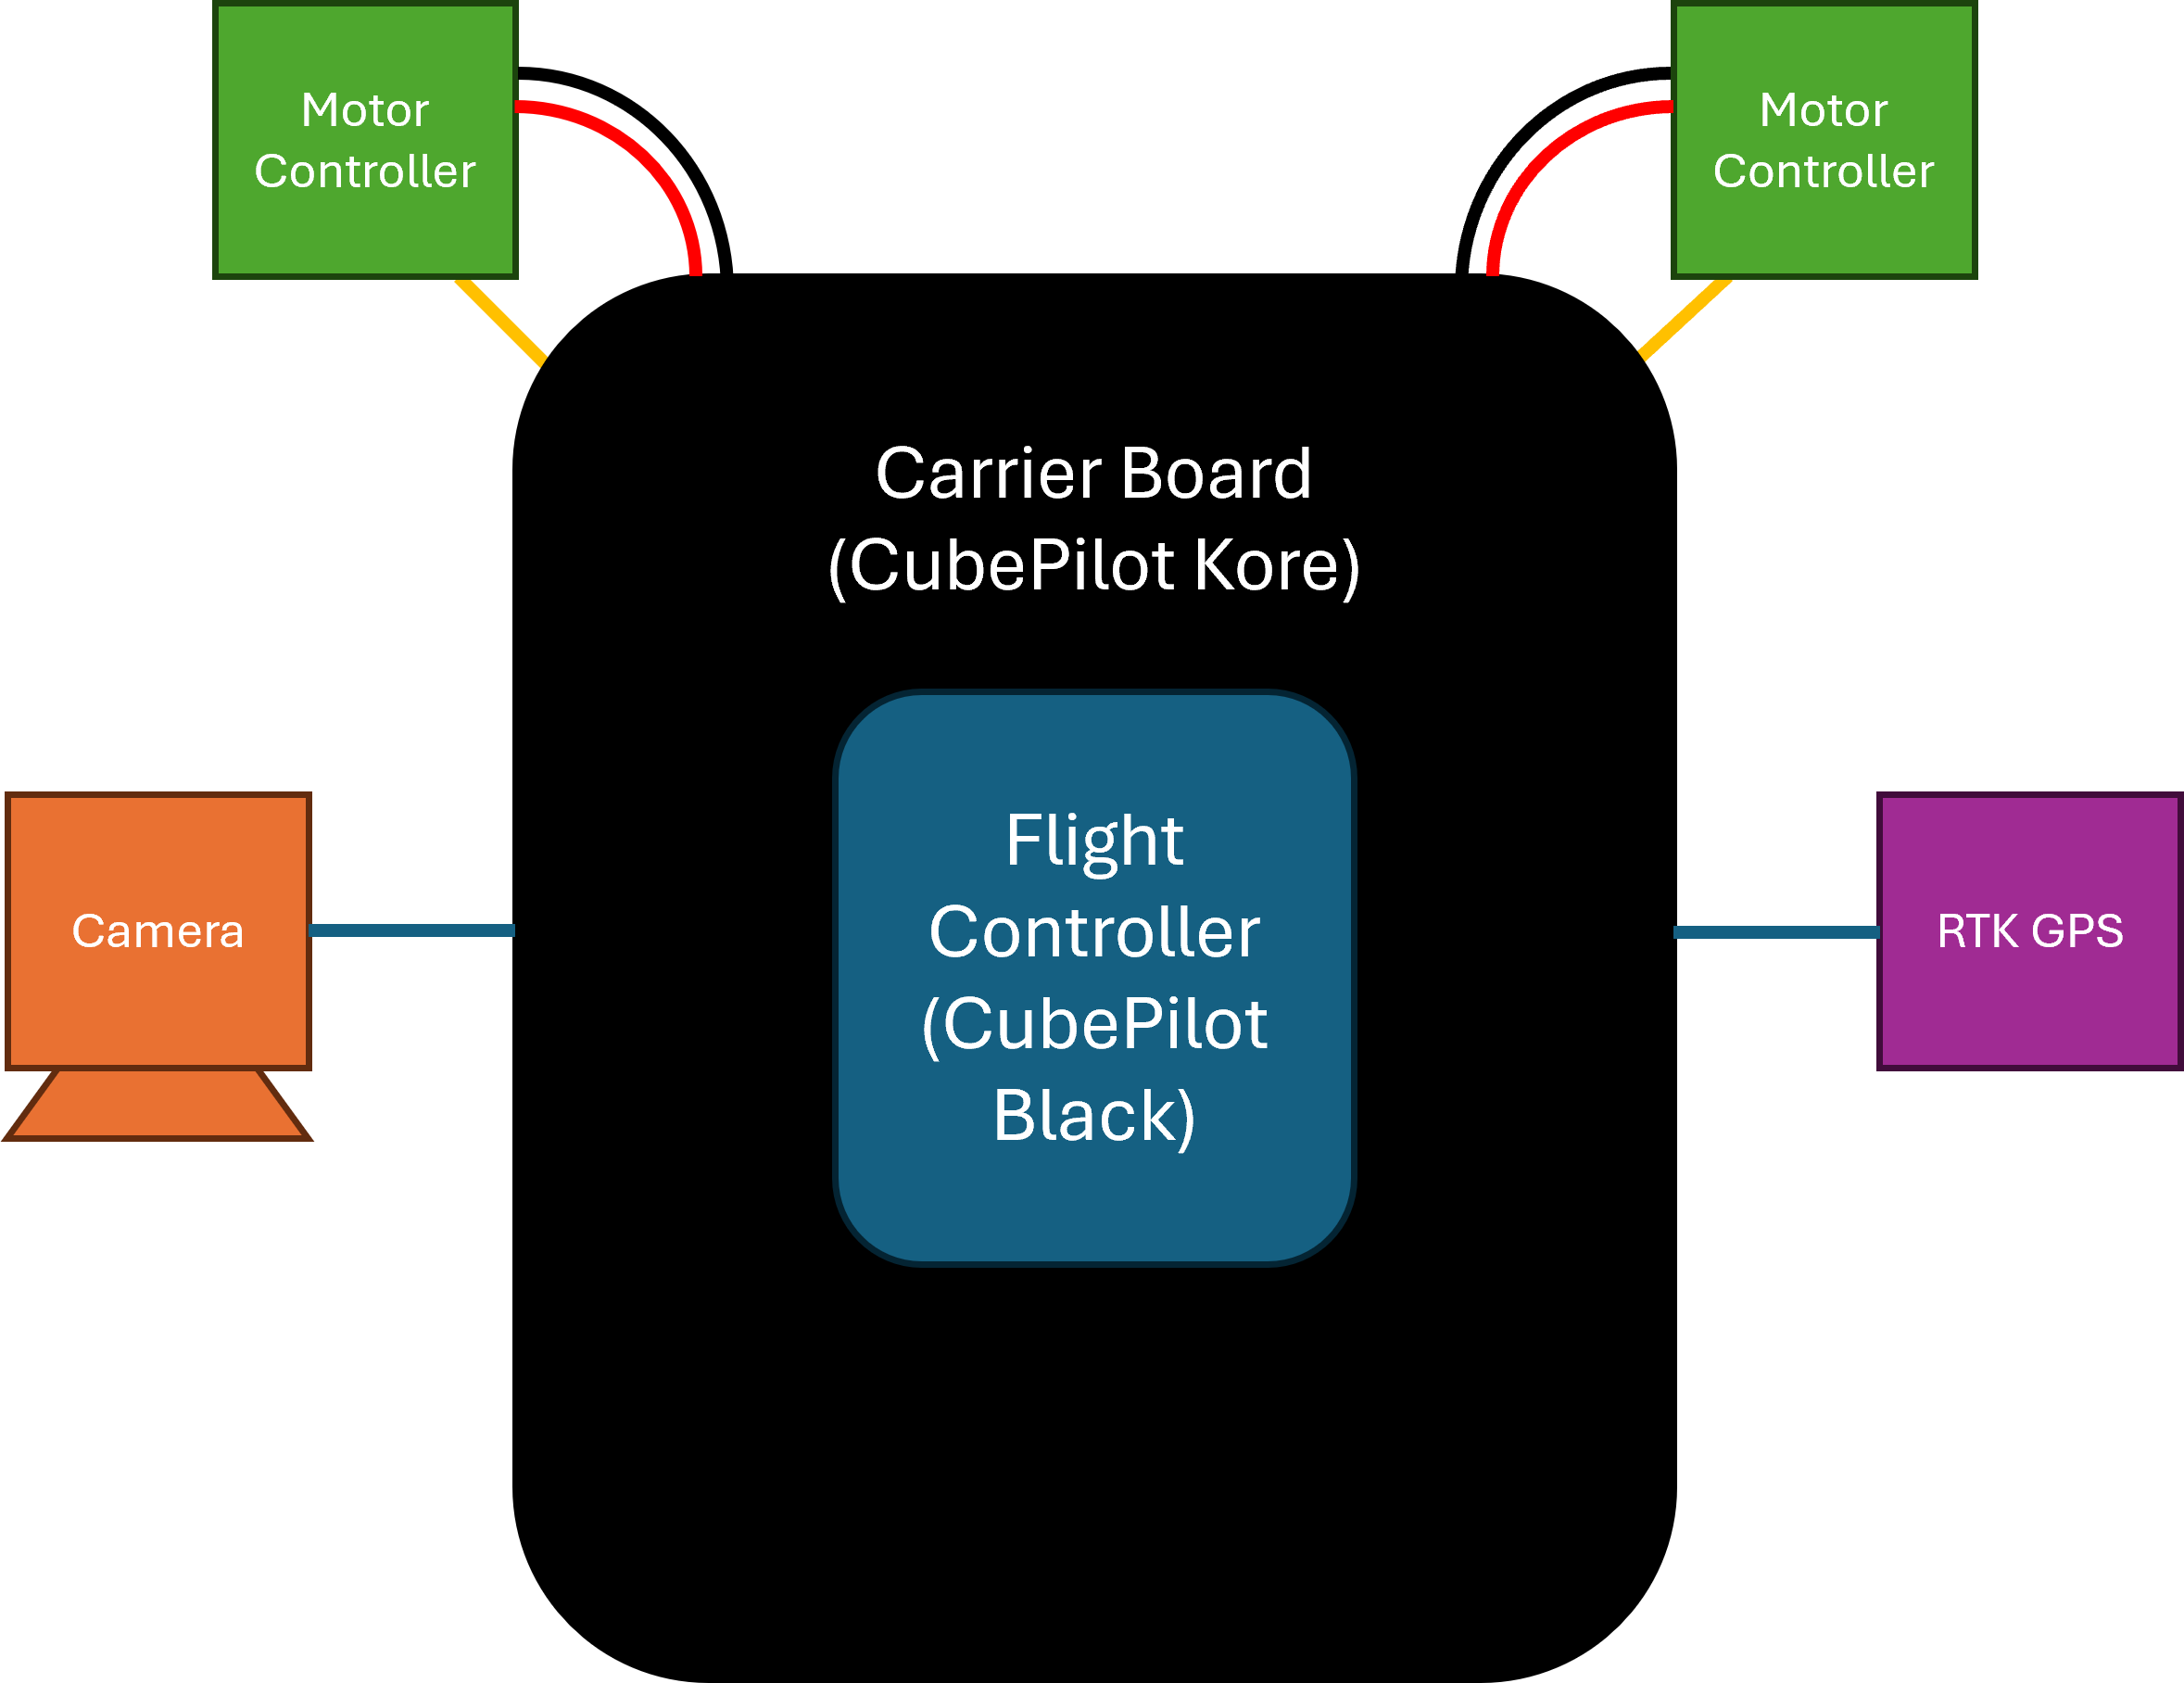
\includegraphics[width=0.75\linewidth]{images/Block_Dia_1.png}
    \caption{System block diagram. Sensors (RGB camera, GNSS/IMU) feed the controller, which handles mission execution and time-stamped image capture. Power distribution, storage, and telemetry are separated into modular subsystems to simplify troubleshooting and field swaps.}
    \label{fig:Block Diagram}
\end{figure}

\section {Bill of materials}

A complete list of materials used, as well as sources and prices at the time of purchase, is listed below.


\begin{table}[!ht]
    \centering
    \caption{Bill of Materials}
    \label{tab:bom}
    \footnotesize
    \begin{tabular}{r l l l c}
        \toprule
        \textbf{Item} & \textbf{Part} & \textbf{Description} & \textbf{Source} & {\textbf{Price (\$)}} \\
        \midrule
        1  & CubePilot Black   & Flight Controller        & IR-LOCK      & 800 \\
        2  & CubePilot Kore    & Carrier Board            & IR-LOCK      & 300 \\
        3  & SparkFun RTK SMA  & RTK GPS Receiver         & IR-LOCK      & 260 \\
        4  & Pololu G2 18v17   & Motor Driver             & Pololu       & 45  \\
        5  & 20 inch Wheels and Hub & Drive Wheel         & Local Source & 85  \\
        6  & Solar Panel       & 100W Renogy Panel        & Amazon       & 125 \\
        7  & Battery           & 50 Ah 12V Battery        & Amazon       & 185 \\
        8  & RC Remote Control & RadioLink T8S            & Amazon       & 55  \\
        9  & Steel             & Tube and Plate for Frame & Local Supply & 180 \\
        10 & Enclosure         & Masterforce 5 gal Tote   & Menards      & 22  \\
        \midrule
        \multicolumn{4}{r}{\textbf{Total}} & {\bfseries 2057} \\
        \bottomrule
    \end{tabular}
\end{table}

\newpage


\section{Conclusion}

Overall the system proved to be robust and able to operate well in real-world field conditions. Traction of the drive system and drive power were more than satisfactory. Additionally, the requirement to operate over extended periods without recharging was found to be well exceeded, with the rover able to complete over three full field samplings without any additional off-site or solar charging. The physical structure of the rover was updated to improve performance as well as increase reliability. Steering was changed from having two systems, rotatable drive wheels and differential steering, to exclusively using the differential steering. While differential steering has been used in many agricultural robots \cite{veiros_multitask_2022} the use of two drive wheels with passive caster wheels for stability offers notable improvements in agility in addition to a decreased risk of crop damage. The primary difficulty found was in accurately navigating between plots and then pivoting at the end of rows in order to move to the next row without excessive navigation over existing crop. This issue could be mitigated by utilizing the rows of buffer areas surrounding the test areas as shown in Figure~\ref{fig:path}. Additionally, damage to any crop or fruit was reduced due to the rover's light weight combined with the large footprint of the pneumatic tires. To improve navigation accuracy, it was determined that further decreasing the gearing between the motors and drive wheels would help to lower the operating speed and allow the motion controller to better correct for errors due to uneven terrain; additionally, the inclusion of closed-loop control over the drive motors may decrease overshoot while maneuvering.

This work showed the potential of an automated image collection system that was cost-effective while still being robust enough for season-long use. The 2-wheel drive configuration exhibited good maneuverability while also simplifying the overall machine layout and minimizing damage to the crop or field due to skidding.  Improvements to the navigation system would increase the usability of the system and allow for the addition of further sensors as well as manipulators to interact with crops as needed.

\newpage

\section{References}

\printbibliography[heading=none]

